\section{Experiments}




\subsection{Experimental Settings}
\textbf{Datasets.} {To evaluate the effectiveness of \method{}, we conduct experiments on two widely used KGQA benchmarks: WebQSP~\cite{talmor2018web} and CWQ~\cite{yih2016value}. Following prior work~\cite{sun2023think,liu2025dual}, we uniformly sample 1,000 questions from the test sets of both datasets to evaluate the performance.} More details about datasets are provided in Appendix ~\ref{sec:dataset}. 



\noindent\textbf{Baselines.} We compare \method{} with a comprehensive set of baselines. These baselines include: the semantic parsing methods, e.g., KV-Mem~\citep{miller2016key}, EmbedKGQA~\citep{saxena2020improving}, QGG~\citep{lan2020query}, NSM~\citep{he2021improving}, TransferNet~\citep{shi2021transfernet}, and KGT5~\citep{saxena2022sequence};
the retrieval-based methods, e.g., GraftNet~\citep{sun2018open}, PullNet~\citep{sun2019pullnet}, SR+NSM~\citep{zhang2022subgraph}, and SR+NSM+E2E~\citep{zhang2022subgraph};
the general LLMs, including 
Flan-T5-xl~\citep{chung2024scaling}, Alpaca-7B~\citep{taori2023stanford},
Llama3-8B~\citep{dubey2024llama}, Qwen2.5-7B~\citep{team2024qwen2}, ChatGPT~\citep{schulman2022chatgpt}, and ChatGPT+CoT~\citep{wei2022chain};
and recent LLMs with KG methods, including UniKGQA~\citep{jiang2022unikgqa},DECAF~\citep{yu2022decaf}, KD-CoT~\citep{wang2023knowledge},
Nutrea~\citep{choi2023nutrea}, ToG~\citep{sun2023think}, RoG~\citep{luo2023reasoning}, KAPING~\citep{baek2023knowledge}, ReasoningLM~\citep{jiang2023reasoninglm},
FiDeLis~\citep{sui2024fidelis}, GNN-RAG~\citep{mavromatis2024gnn},
DoG~\citep{ma2025debate},  DualR~\citep{liu2025dual}
, DP~\citep{ma2025deliberation}, and RwT~\citep{shen2025reasoning}. The details are provided in Appendix~\ref{sec:baseline}.

% \noindent\textbf{Evaluation Metric.} Following~\citep{luo2023reasoning,yao2025learning,ma2025deliberation}, we evaluate \method{} using Hits@1 and F1 score, assessing answer correctness and overall accuracy for questions with potentially multiple correct answers.
\begin{table*}[t]
\centering
\small
\begin{tabular}{clcccc}
\toprule
\multirow{2}{*}{\textbf{Type}} 
& \multirow{2}{*}{\textbf{Methods}} 
& \multicolumn{2}{c}{\textbf{WebQSP}} 
& \multicolumn{2}{c}{\textbf{CWQ}} \\
& & Hits@1 & F1 & Hits@1 & F1 \\
\midrule
\multirow{6}{*}{Semantic Parsing} 
& KV-Mem~\citep{miller2016key} & 46.7 & 34.5 & 18.4 & 15.7 \\
& EmbedKGQA~\citep{saxena2020improving} & 66.6 & - & 45.9 & - \\
& QGG~\citep{lan2020query} & 73.0 & 73.8 & 36.9 & 37.4 \\
& NSM~\citep{he2021improving} & 68.7 & 62.8 & 47.6 & 42.4 \\
& TransferNet~\citep{shi2021transfernet} & 71.4 & - & 48.6 & - \\
& KGT5~\citep{saxena2022sequence} & 56.1 & - & 36.5 & - \\
\midrule
\multirow{4}{*}{Retrieval} 
& GraftNet~\citep{sun2018open} & 66.4 & 60.4 & 36.8 & 32.7 \\
& PullNet~\citep{sun2019pullnet} & 68.1 & - & 45.9 & - \\
& SR+NSM~\citep{zhang2022subgraph} & 68.9 & 64.1 & 50.2 & 47.1 \\
& SR+NSM+E2E~\citep{zhang2022subgraph} & 69.5 & 64.1 & 49.3 & 46.3 \\
\midrule
\multirow{6}{*}{LLMs} 
& Flan-T5-xl~\cite{chung2024scaling} & 31.0 & - & 14.7 & - \\
& Alpaca-7B~\cite{taori2023stanford} & 51.8 & - & 27.4 & - \\
& Llama3-8B~\citep{dubey2024llama} & 30.3 & 25.7 & 30.5 & 27.8 \\
& Qwen2.5-7B~\citep{team2024qwen2} & 28.4 & 23.7 & 25.9 & 24.1 \\
& ChatGPT~\citep{schulman2022chatgpt} & 66.8 & - & 39.9 & - \\
& ChatGPT+CoT~\citep{wei2022chain} & 75.6 & - & 48.9 & - \\
\midrule
\multirow{13}{*}{LLMs+KGs} 
& UniKGQA~\citep{jiang2022unikgqa} & 77.2 & 72.2 & 51.2 & 49.0 \\
& DECAF~\cite{yu2022decaf} & 82.1 & 78.8 & 70.4 & - \\
& KD-CoT~\cite{wang2023knowledge} & 68.6 & 52.5 & 55.7 & - \\
& Nutrea~\citep{choi2023nutrea} & 77.4 & 72.7 & 53.6 & 49.5 \\
& ToG~\citep{sun2023think} & 81.9 & 76.0 & 68.5 & 60.2 \\
& RoG~\citep{luo2023reasoning} & 80.8 & 70.8 & 57.8 & 56.2 \\
& KAPING~\citep{baek2023knowledge} & 72.4 & 65.1 & 53.4 & 50.3 \\
& ReasoningLM~\citep{jiang2023reasoninglm} & 78.5 & 71.0 & 69.0 & 64.0 \\
& FiDeLis~\citep{sui2024fidelis} & 84.3 & 78.3 & 71.5 & 64.3 \\
& GNN-RAG~\citep{mavromatis2024gnn} & 82.8 & 73.5 & 62.8 & 60.4 \\
& DoG~\citep{ma2025debate} & 65.4 & 55.6 & 41.0 & 46.4 \\
& DualR~\citep{liu2025dual} & 81.5 & 71.6 & 65.3 & 62.1 \\
& DP~\citep{ma2025deliberation} & {87.5} & {81.4} & {75.8} & {69.4} \\
& RwT~\citep{shen2025reasoning} & 87.0 & 79.7 & 72.4 & 66.7 \\
\midrule
& \method{} & \textbf{94.0} & \textbf{81.7} & \textbf{78.0} & \textbf{75.1} \\
\bottomrule
\end{tabular}
\vspace{-2pt}
\caption{Performance comparison (\%) on WebQSP and CWQ datasets. \textbf{Bold} results indicate the best performance.}

\label{tab:main_results}
\end{table*}

\noindent\textbf{Implementation Details.} We implement the DAMR framework using PyTorch, and all experiments are conducted on NVIDIA A100 GPUs. The LLM-based planner is implemented with GPT-4.1~\citep{liu2023evaluating}, while question and relation embeddings are generated from Qwen3-Embedding-8B~\citep{yang2025qwen3} with an embedding dimension of 1024. For the path evaluation module, we use a 128-dimensional embedding and employ the Adam optimizer~\citep{kingma2014adam} with a learning rate of $1\times10^{-4}$ during pretraining and $1 \times 10^{-5}$ during fine-tuning. The model consists of two Transformer layers and is trained for 15 epochs in the pretraining stage and 10 epochs in the fine-tuning stage. Following~\citep{luo2023reasoning,yao2025learning,ma2025deliberation}, we evaluate \method{} using Hits@1 and F1 score, assessing answer correctness and overall accuracy for questions with potentially multiple correct answers.



\subsection{Performance Comparison}

We report the experimental results of \method{} in Table~\ref{tab:main_results}, benchmarking its performance against state-of-the-art baselines across KGQA datasets. From the results, we find that: 
% (1) Semantic parsing and retrieval-based methods provide a foundational backbone for KGQA by capturing structural semantics and retrieving relevant subgraphs from large-scale knowledge bases. While embedding-based models encode entity and relation representations, they often fall short in modeling complex relational dependencies and multi-hop reasoning patterns. Retrieval-based approaches offer richer contextual signals through explicit subgraph construction, enhancing reasoning over relevant neighborhoods. However, their dependence on pre-defined retrieval pipelines restricts adaptability to evolving query semantics. 
(1) Semantic parsing and retrieval-based methods serve as early foundations for KGQA by extracting subgraphs and capturing structural semantics. However, embedding-based models struggle with complex relational patterns, while retrieval-based methods rely on rigid pipelines that limit generalization. In contrast, LLM with KG approaches combine the language understanding of LLMs with structured reasoning over KGs, enabling more flexible path exploration and improved adaptability to diverse, multi-hop queries.
(2) General-purpose LLMs, such as ChatGPT and Llama3-8B, show basic reasoning ability but often perform worse than methods that combine LLMs with KGs in KGQA tasks. This is mainly because they are not grounded in domain-specific knowledge, making them more likely to produce incorrect or made-up answers. 
% (2) LLMs with KG methods significantly enhance reasoning effectiveness by integrating LLMs and structured relational knowledge. The inclusion of graph-based entity and relation embeddings enables these methods to capture richer semantic relationships and more effectively handle complex multi-hop queries. Consequently, these methods approaches consistently outperform general LLMs across both datasets. 
(3) \method{} consistently outperforms all baselines across both datasets, showcasing its strong reasoning capability. This superior performance is driven by its integration of an LLM-based planner, which selectively retrieves relevant relations to reduce noise and guide the search toward high-quality reasoning paths, and a path evaluation model that is dynamically fine-tuned during search to capture semantic differences among candidate paths and accurately rank those most likely to yield correct answers.


\vspace{-1pt}
\subsection{Efficiency Analysis}
As shown in Table~\ref{tab:Efficiency}, \method{} achieves substantial improvements in computational efficiency. It reduces the average number of LLM calls to 7.1 on WebQSP and 16.8 on CWQ, with corresponding token usage of 3,931 and 9,266. These correspond to reductions of over 50\% in LLM calls and 75\% in token consumption relative to the strongest baseline. This efficiency is achieved by invoking the LLM only during the expansion phase of MCTS to select the top-$k$ semantically relevant relations, which effectively narrows the search space and avoids redundant reasoning steps that lead to unnecessary computational overhead. During simulation, the context-aware path evaluator efficiently assesses candidate paths based on question-path alignment without requiring any further LLM interaction or model inference. These design choices reduce both the frequency and verbosity of LLM usage while maintaining strong reasoning performance, making \method{} more efficient, scalable, and practically deployable than previous work.

% To assess the computational efficiency of \method{}, we evaluate its average number of LLM calls and token consumption per question on the WebQSP and CWQ datasets. As shown in Table~\ref{tab:Efficiency}, \method{} significantly reduces both LLM calls and token usage compared to baselines such as DoG~\citep{ma2025debate}, ToG~\citep{luo2023reasoning}, and RwT~\citep{shen2025reasoning}. Specifically, \method{} lowers the average number of LLM calls to 7.1 on WebQSP and 16.8 on CWQ, achieving over a 50\% reduction relative to the most efficient baseline. Similarly, it reduces token consumption by more than 75\% on both datasets. These results demonstrate the superior efficiency of \method{}, making it considerably more practical and cost-effective for real-world deployment.



\subsection{Ablation Study}\label{sec:ablation}

We conduct ablation studies to assess the contributions of key components in \method{}: (1) \method{} w/o PE: removing the path evaluation module; (2) \method{} w/o FT: disabling fine-tuning of the evaluator; and (3) \method{} w/ GPT-4.1: replacing the context-aware evaluator with a general LLM.

Experimental results are summarized in Table~\ref{tab:ablation_results}. From the results, we find that:
(1) Removing the path evaluation module (\method{} w/o PE) causes a noticeable performance drop on both datasets, underscoring its critical role in guiding the search process. Without this component, the model cannot effectively assess or rank candidate paths, leading to suboptimal reasoning and reduced accuracy.
(2) Compared to \method{} w/o FT, the proposed \method{} consistently achieves superior results on both datasets, highlighting the importance of the finetuning mechanism in the path evaluation module. This mechanism enables the model to adapt to the evolving distribution of explored paths, improving its ability to distinguish plausible from implausible reasoning trajectories.
(3) Replacing the context-aware path evaluation module with general LLMs yields degraded performance, confirming the advantage of our fine-tuned path scorer. By capturing fine-grained semantic distinctions among candidate paths, it provides more accurate evaluation signals, enhancing overall search effectiveness.

% \begin{table}[t]
% \centering
% \small
% \begin{tabular}{l|cc|cc}
% \toprule
% \multirow{2}{*}{Method} & \multicolumn{2}{c}{WebQSP} & \multicolumn{2}{c}{CWQ} \\
%  & Hits@1 & F1 & Hits@1 & F1 \\
% \midrule

% \method{} w/o PE & 91.2 & 78.2 & 74.3 & 72.1 \\

% \method{} w/o FT & 91.9 & 80.1 & 75.1 & 73.0 \\

% \method{} w/ GPT 4.1 & 92.5 & 79.8 & 74.9 & 72.4 \\

% % \method{} w GPT 4.1-mini & 92.9 & 80.1 & 75.4 & 72.8 \\

% % \method{} w Llama2-13B & 92.0 & 78.8 & 75.2 & 72.5 \\

% % \method{} w Qwen3-14B & 92.3 & 79.2 & 75.7 & 73.3 \\

% \midrule

% \method{} & \textbf{94.0} & \textbf{81.7} & \textbf{78.0} & \textbf{75.1} \\

% \bottomrule
% \end{tabular}
% \caption{The results of ablation studies on the WebQSP and CWQ datasets. \textbf{Bold} results indicate the best performance.}
% \label{tab:ablation_results}
% \end{table}

\begin{table}[t]
\centering
\begin{minipage}{\textwidth}
\begin{minipage}[t]{0.47\textwidth}
\makeatletter\def\@captype{table}
\centering
\footnotesize
\tabcolsep=3pt
\begin{tabular}{l@{\hspace{2em}}|cc|cc}
\toprule
\multirow{2}{*}{Method} & \multicolumn{2}{c|}{WebQSP} & \multicolumn{2}{c}{CWQ} \\
 & \#Tokens & \#Calls & \#Tokens & \#Calls \\
\midrule
DoG       & 22,538 & 30.9  & 37,741 & 58.1 \\
ToG       & 16,372 &  23.2 & 26,183 & 41.9 \\
RwT       & 10,680 & 15.1 & 17,885 &  28.6 \\
\midrule
\method{} &  \textbf{3,931} & \textbf{7.1} &  \textbf{9,266} &  \textbf{16.8} \\
\bottomrule
\end{tabular}
\vspace{0.5cm}
\caption{Statistics of average number of LLM calls and token consumption per question on WebQSP and CWQ datasets.}
\label{tab:Efficiency}
\end{minipage}
\hspace{0.18in}
\begin{minipage}[t]{0.48\textwidth}
\makeatletter\def\@captype{table}
\centering
\footnotesize
\tabcolsep=3pt
\begin{tabular}{l|cc|cc}
\toprule
\multirow{2}{*}{Method} & \multicolumn{2}{c}{WebQSP} & \multicolumn{2}{c}{CWQ} \\
 & Hits@1 & F1 & Hits@1 & F1 \\
\midrule

\method{} w/o PE & 91.2 & 78.2 & 74.3 & 72.1 \\

\method{} w/o FT & 91.9 & 80.1 & 75.1 & 73.0 \\

\method{} w/ GPT 4.1 & 92.5 & 79.8 & 74.9 & 72.4 \\

% \method{} w GPT 4.1-mini & 92.9 & 80.1 & 75.4 & 72.8 \\

% \method{} w Llama2-13B & 92.0 & 78.8 & 75.2 & 72.5 \\

% \method{} w Qwen3-14B & 92.3 & 79.2 & 75.7 & 73.3 \\

\midrule

\method{} & \textbf{94.0} & \textbf{81.7} & \textbf{78.0} & \textbf{75.1} \\

\bottomrule
\end{tabular}
\vspace{0.5cm}
\caption{The results of ablation studies on the WebQSP and CWQ datasets. \textbf{Bold} results indicate the best performance.}
\label{tab:ablation_results}
\end{minipage}
\end{minipage}
\vspace{-0.5cm}
\end{table}


\begin{wrapfigure}{r}{0.6\textwidth}
\vspace{-0.9cm}
\begin{minipage}[t]{0.6\textwidth}
        \centering
        \hspace{-1cm}
    \subfloat[Number of selected relations $k$]{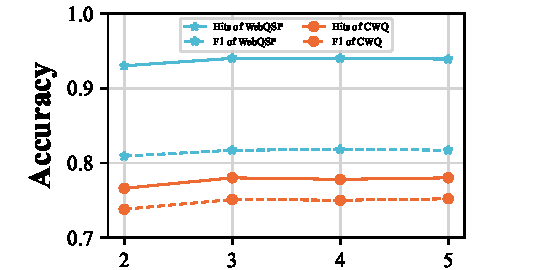
\includegraphics[width=0.53\textwidth,height=0.29\textwidth]{figure/hyper_top_k.pdf}}
    \label{fig:mcts_top_k}
    \hspace{-0.5cm}
    \subfloat[Reasoning path length $L$]{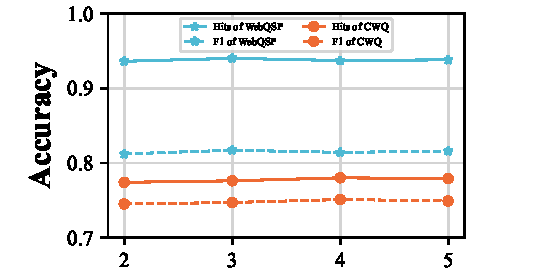
\includegraphics[width=0.53\textwidth,height=0.29\textwidth]{figure/hyper_mcts_deep.pdf}}
    \label{fig:mcts_length}
    \hspace{-1.3cm}
    \vspace{-0.2cm}
    \caption{Sensitivity analysis of hyperparameter on the WebQSP and CWQ datasets.}
        \label{fig:hyper_sensitive}
    \end{minipage}%
    \vspace{-0.4cm}
\end{wrapfigure}


\subsection{Sensitivity Analysis}\label{sec:sensitivity}

We conduct a sensitivity analysis to assess the impact of two key hyperparameters in \method{}: the number of selected relations $k$ and the maximum reasoning path length $L$. The parameter $k$ controls how many relations are proposed by the LLM-based planner at each step, while $L$ determines the number of reasoning hops allowed during path construction.

Figure \ref{fig:hyper_sensitive} illustrates how $k$ and  $L$ affect the performance of \method{} on the WebQSP and CWQ datasets. We vary $k$ and $L$ within the range of  $\{2, 3, 4, 5\}$. From the results, we observe that: (1) As shown in Figure~\ref{fig:hyper_sensitive}(a), increasing $k$ initially leads to performance gains, which then stabilize before experiencing a slight decline. While larger $k$ values encourage broader relational exploration, they may also introduce irrelevant candidates and increased computational cost. Conversely, smaller $k$ restrict the diversity of the search. To balance these trade-offs, we select a moderate $k=3$ as the default setting. (2) As shown in Figure~\ref{fig:hyper_sensitive}(b), on the WebQSP dataset, performance improves from $L=2$ to $3$, then fluctuates between $L=3$ and $5$, suggesting limited gains beyond three hops. In contrast, performance on the CWQ dataset steadily increases up to $L=4$ before slightly declining at $L=5$, reflecting its need for deeper reasoning due to more complex questions. Balancing effectiveness and efficiency across both datasets, we set $L=4$ as the default path length in all experiments. 
More results are provided in Appendix ~\ref{sec:experiments_results}.





% \vspace{-5pt}
\subsection{Impact of Different LLMs} 
\begin{wraptable}{r}{0.6\textwidth} 
\vspace{-29pt}
\footnotesize
\centering
\tabcolsep=6pt
\begin{tabular}{l|cc|cc}
\toprule
\multirow{2}{*}{Method} & \multicolumn{2}{c}{WebQSP} & \multicolumn{2}{c}{CWQ} \\
 & Hits@1 & F1 & Hits@1 & F1 \\
\midrule
\method{} (Llama2-13B) & 91.0 & 76.7 & 73.9 & 69.5 \\
\method{} (Qwen3-14B) & 91.5 & 77.8 & 74.4 & 70.1 \\
\method{} (GPT 4.1-mini) & 93.1 & 80.6 & 76.1 & 72.7 \\
\method{} (GPT 4.1) & \textbf{94.0} & \textbf{81.7} & \textbf{78.0} & \textbf{75.1} \\
\bottomrule
\end{tabular}
            % \caption{Example Table}
            \caption{Performance of \method{} using different LLM-based planners as backbones on different datasets.}\label{tab:backbone_results}
\end{wraptable}
To evaluate the impact of different LLM-based planners within the \method{} framework, we compare several backbones including Llama2-13B~\citep{roque2025evolution}, Qwen3-14B~\citep{team2024qwen2}, GPT 4.1 mini, and GPT 4.1, as shown in Table~\ref{tab:backbone_results}. Across both datasets, stronger LLMs consistently yield higher F1 and Hits scores, with GPT 4.1 achieving the best performance across all metrics. These results highlight the pivotal role of advanced LLMs in guiding relation selection and reasoning path expansion, where improved fluency, contextual awareness, and semantic precision translate into more accurate and faithful reasoning trajectories. Notably, the consistent performance gap between smaller and larger backbones illustrates the sensitivity of KGQA systems to the planner’s reasoning capability, reinforcing the necessity of leveraging high-capacity models when available. Overall, these findings emphasize the importance of backbone selection and further validate the design of \method{}, which capitalizes on powerful LLMs to achieve robust, generalizable, and effective multi-hop reasoning.

% \begin{figure*}[t]
%     \centering
%     % 左侧：图片
%     \begin{minipage}[t]{0.48\textwidth}
%         \centering
%         \hspace{-1cm}
%     \subfloat[Number of selected relations $k$]{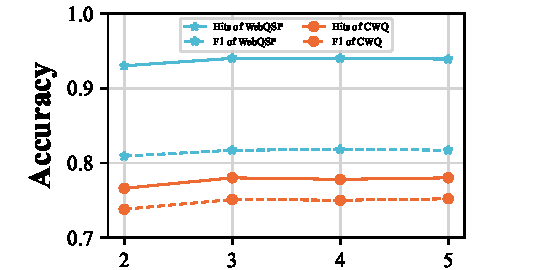
\includegraphics[width=0.53\textwidth,height=0.29\textwidth]{figure/hyper_top_k.pdf}}
%     \label{fig:mcts_top_k}
%     \hspace{-0.5cm}
%     \subfloat[Reasoning path length $L$]{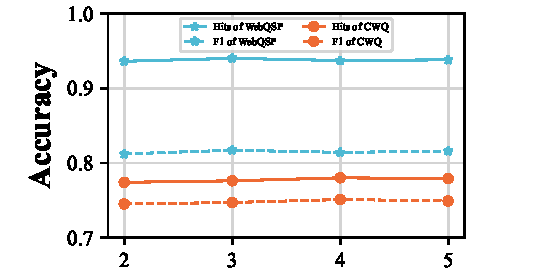
\includegraphics[width=0.53\textwidth,height=0.29\textwidth]{figure/hyper_mcts_deep.pdf}}
%     \label{fig:mcts_length}
%     \hspace{-1.3cm}

%     \caption{ Sensitivity analysis of hyperparameter on the WebQSP and CWQ datasets.}
%         \label{fig:hyper_sensitive}
%     \end{minipage}%
%     \hfill
%     % 右侧：表格
%     \begin{minipage}[t]{0.48\textwidth}
%     \vspace{-2.9cm}
%         \centering
        
%         \begin{table}[H] % 使用 [H] 防止表格浮动，需 \usepackage{float}
%             \centering
%             \small
%             % \setlength{\tabcolsep}{7pt}
% \begin{tabular}{l|cc|cc}
% \toprule
% \footnotesize
% \tabcolsep=5pt
% \multirow{2}{*}{Method} & \multicolumn{2}{c}{WebQSP} & \multicolumn{2}{c}{CWQ} \\
%  & Hits@1 & F1 & Hits@1 & F1 \\
% \midrule

% \method{} (Llama2-13B) & 91.0 & 76.7 & 73.9 & 69.5 \\

% \method{} (Qwen3-14B) & 91.5 & 77.8 & 74.4 & 70.1 \\

% \method{} (GPT 4.1-mini) & 93.1 & 80.6 & 76.1 & 72.7 \\

% \method{} (GPT 4.1) & \textbf{94.0} & \textbf{81.7} & \textbf{78.0} & \textbf{75.1} \\

% \bottomrule
% \end{tabular}
%             % \caption{Example Table}
%             \caption{Performance of \method{} using different LLM-based planners as backbones on the WebQSP and CWQ datasets. \textbf{Bold} values denote the best results.}\label{tab:backbone_results}
%         \end{table}
%     \end{minipage}
% \end{figure*}


% \begin{table*}[t]
% \renewcommand{\arraystretch}{1.3}
% \small
% \centering
% % \vspace{-0.1cm}
% \begin{tabular}{>{\centering\arraybackslash}m{2.5cm}|p{7.6cm}}
% \toprule
% \textbf{Question} & What structure opened in 1922 in Hollywood, CA? \\
% \hline
% \textbf{Answer} & \textcolor{red}{Grauman's Egyptian Theatre} \\
% \hline
% \multirow{4}{*}{\textbf{Llama-2-13B}} & \textcolor{blue}{The Grauman's Chinese Theatre}, a historic movie palace, opened on November 18, 1922, in Hollywood, CA. It was built by Sid Grauman and Charles E. Toberman and has since become a famous landmark and tourist attraction. \\
% \hline
% \multirow{4}{*}{\textbf{Qwen-3-14B}} & \textcolor{blue}{The TCL Chinese Theatre}, originally known as the Chinese Grand Theatre, opened in 1922 in Hollywood, CA. It is a historic movie theater renowned for its unique architecture and celebrity handprints and footprints. \\
% \hline
% \multirow{3}{*}{\textbf{GPT 4.1}} & \textcolor{blue}{The Hollywood Bowl}, an iconic amphitheater in Hollywood, California, opened in 1922. It is renowned for its distinctive band shell and has hosted numerous concerts and events, becoming a significant cultural landmark in the area. \\
% \hline
% \multirow{3}{*}{\textbf{GPT 4.1-mini}} & \textcolor{blue}{The Hollywood Bowl}, an iconic amphitheater in Hollywood, California, opened in 1922 and has since been a renowned venue for music performances and cultural events. \\
% \hline
% \multirow{7}{*}{\textbf{\method{}}} & \texttt{Path 1}: Entity (id: 83076) $\rightarrow$ location.location.events $\rightarrow$ time.event.locations $\rightarrow$ travel.travel\_destination.tourist\_attractions $\rightarrow$ \textcolor{red}{Grauman's Egyptian Theatre}.  

% \texttt{Path 2}: Entity (id: 83076) $\rightarrow$ travel.travel\_destination.tourist\_attractions $\rightarrow$ \textcolor{red}{Grauman's Egyptian Theatre}. \\
% \bottomrule
% \end{tabular}
% \caption{Case study of \method{}. We highlight the correct answers in \textcolor{red}{Red} and the wrong answers in \textcolor{blue}{Blue}.}
% \label{tab:case_study_method}
% \vspace{-0.4cm}
% \end{table*}


\begin{figure}[t]
    \centering
    \subfloat[One example from the WebQSP dataset.]{
    \label{fig:webqsp}    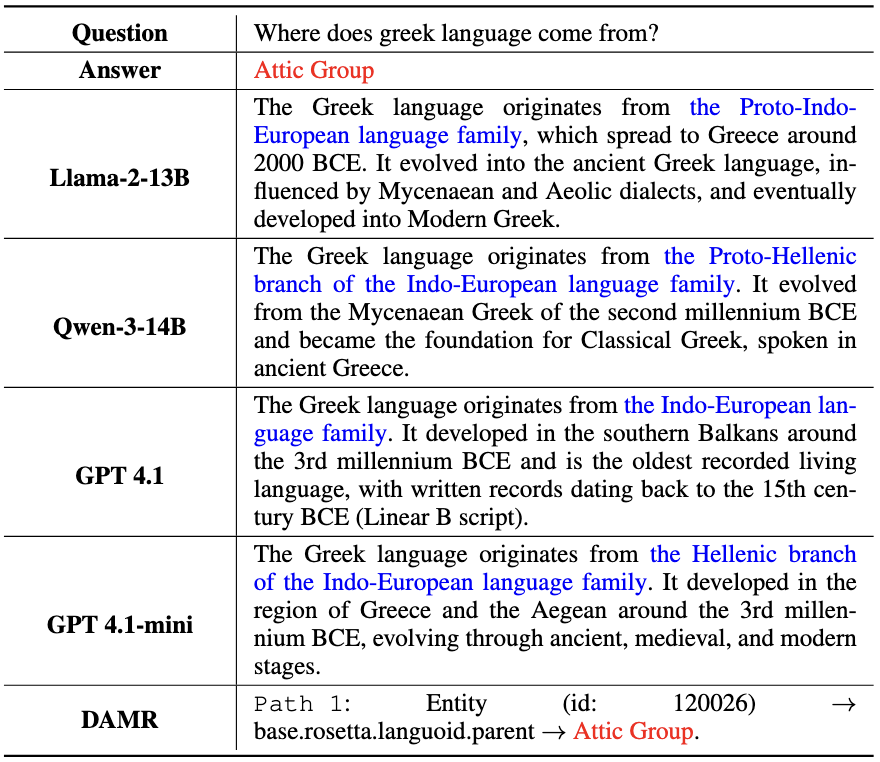
\includegraphics[width=0.47\linewidth]{figure/case_study_1.png}
    }
    \hspace{0.02\linewidth}
    \subfloat[One example from the CWQ dataset.]{
        \label{fig:cwq} 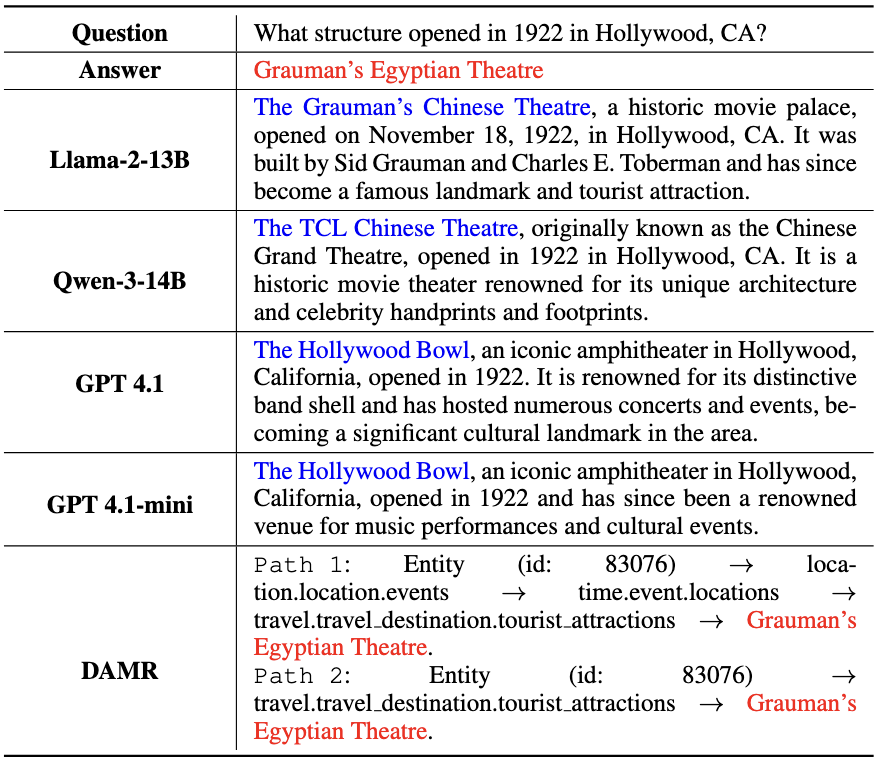
\includegraphics[width=0.47\linewidth]{figure/case_study_2.png}
    }
    \caption{Case studies of \method{} on the WebQSP and CWQ datasets. We highlight the correct answers in \textcolor{red}{Red} and the wrong answers in \textcolor{blue}{Blue}.}
    \label{fig:two_side_by_side}
\end{figure}




\subsection{Case study}

{Figure~\ref{fig:two_side_by_side} presents detailed case studies on the WebQSP and CWQ datasets comparing the reasoning process of \method{} with four representative LLMs: Llama-2-13B, Qwen-3-14B, GPT 4.1-mini, and GPT 4.1. In Figure~\ref{fig:webqsp}, the baseline LLMs generate fluent and seemingly plausible answers such as “Proto-Indo-European” or “Proto-Hellenic” when asked about the origin of the Greek language, yet fail to identify the correct answer \texttt{Attic Group}. In contrast, \method{} accurately predicts the correct entity by explicitly traversing the \textit{base.rosetta.languoid.parent} relation within the knowledge graph. In Figure~\ref{fig:cwq}, none of the baseline models are able to identify the structure that opened in Hollywood in 1922, while the proposed \method{} successfully locates \texttt{Grauman’s Egyptian Theatre} by explicitly following relevant relation paths in the knowledge graph and integrating complementary reasoning trajectories. These examples collectively highlight the strength of \method{} in grounding its reasoning in the knowledge graph and explicitly modeling multi-step reasoning paths, enabling it to provide accurate and faithful answers to complex, ontology-specific questions that general-purpose LLMs often struggle to resolve.}
% Figure~\ref{fig:two_side_by_side} presents detailed case studies on the WebQSP and CWQ datasets comparing the reasoning process of \method{} with four representative LLMs: Llama-2-13B, Qwen-3-14B, GPT 4.1-mini, and GPT 4.1. While all baseline LLMs fail to identify the correct structure that opened in Hollywood in 1922, the proposed \method{} accurately finds \texttt{Grauman’s Egyptian Theatre} by explicitly traversing relation paths in the knowledge graph through two complementary reasoning paths. This example illustrates that, although LLMs may appear capable of answering the question, their responses can nevertheless be factually incorrect due to the absence of grounded knowledge. In contrast, \method{} consistently produces more accurate and faithful answers by grounding its reasoning in the KG and explicitly modeling reasoning trajectories.


% \begin{figure}[t]
%     \centering
%     \hspace{-1.0cm}
%     \subfloat[Number of selected relations $k$]{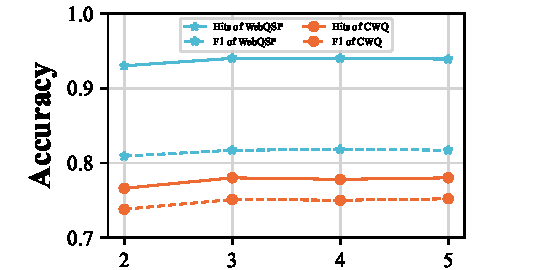
\includegraphics[width=0.265\textwidth,height=0.145\textwidth]{figure/hyper_top_k.pdf}}
%     \label{fig:mcts_top_k}
%     \hspace{-0.5cm}
%     \subfloat[Reasoning path length $L$]{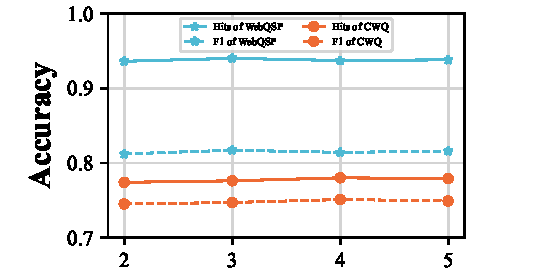
\includegraphics[width=0.265\textwidth,height=0.145\textwidth]{figure/hyper_mcts_deep.pdf}}
%     \label{fig:mcts_length}
%     \hspace{-1.3cm}

%     \caption{ Sensitivity analysis of hyperparameter on the WebQSP and CWQ datasets.}
%     \label{fig:hyper_sensitive}
%     \vspace{-0.4cm}
% \end{figure}

% \begin{table}[t]
% \centering
% \small
% \vspace{-0.1cm}
% \caption{Performance of \method{} using different LLM-based planners as backbones on the WebQSP and CWQ datasets. \textbf{Bold} values denote the best results.}
% \begin{tabular}{l|cc|cc}
% \toprule
% \multirow{2}{*}{Method} & \multicolumn{2}{c}{WebQSP} & \multicolumn{2}{c}{CWQ} \\
%  & Hits@1 & F1 & Hits@1 & F1 \\
% \midrule

% \method{} (Llama2-13B) & 91.0 & 76.7 & 73.9 & 69.5 \\

% \method{} (Qwen3-14B) & 91.5 & 77.8 & 74.4 & 70.1 \\

% \method{} (GPT 4.1-mini) & 93.1 & 80.6 & 76.1 & 72.7 \\

% \method{} (GPT 4.1) & \textbf{94.0} & \textbf{81.7} & \textbf{78.0} & \textbf{75.1} \\

% \bottomrule
% \end{tabular}
% \vspace{-0.4cm}
% \label{tab:backbone_results}
% \end{table}

